% Options for packages loaded elsewhere
\PassOptionsToPackage{unicode}{hyperref}
\PassOptionsToPackage{hyphens}{url}
\documentclass[
  preprint,review,1p,authoryear]{article}
\usepackage{xcolor}
\usepackage[margin=1in]{geometry}
\usepackage{amsmath,amssymb}
\setcounter{secnumdepth}{5}
\usepackage{iftex}
\ifPDFTeX
  \usepackage[T1]{fontenc}
  \usepackage[utf8]{inputenc}
  \usepackage{textcomp} % provide euro and other symbols
\else % if luatex or xetex
  \usepackage{unicode-math} % this also loads fontspec
  \defaultfontfeatures{Scale=MatchLowercase}
  \defaultfontfeatures[\rmfamily]{Ligatures=TeX,Scale=1}
\fi
\usepackage{lmodern}
\ifPDFTeX\else
  % xetex/luatex font selection
\fi
% Use upquote if available, for straight quotes in verbatim environments
\IfFileExists{upquote.sty}{\usepackage{upquote}}{}
\IfFileExists{microtype.sty}{% use microtype if available
  \usepackage[]{microtype}
  \UseMicrotypeSet[protrusion]{basicmath} % disable protrusion for tt fonts
}{}
\makeatletter
\@ifundefined{KOMAClassName}{% if non-KOMA class
  \IfFileExists{parskip.sty}{%
    \usepackage{parskip}
  }{% else
    \setlength{\parindent}{0pt}
    \setlength{\parskip}{6pt plus 2pt minus 1pt}}
}{% if KOMA class
  \KOMAoptions{parskip=half}}
\makeatother
\usepackage{longtable,booktabs,array}
\newcounter{none} % for unnumbered tables
\usepackage{calc} % for calculating minipage widths
% Correct order of tables after \paragraph or \subparagraph
\usepackage{etoolbox}
\makeatletter
\patchcmd\longtable{\par}{\if@noskipsec\mbox{}\fi\par}{}{}
\makeatother
% Allow footnotes in longtable head/foot
\IfFileExists{footnotehyper.sty}{\usepackage{footnotehyper}}{\usepackage{footnote}}
\makesavenoteenv{longtable}
\usepackage{graphicx}
\makeatletter
\newsavebox\pandoc@box
\newcommand*\pandocbounded[1]{% scales image to fit in text height/width
  \sbox\pandoc@box{#1}%
  \Gscale@div\@tempa{\textheight}{\dimexpr\ht\pandoc@box+\dp\pandoc@box\relax}%
  \Gscale@div\@tempb{\linewidth}{\wd\pandoc@box}%
  \ifdim\@tempb\p@<\@tempa\p@\let\@tempa\@tempb\fi% select the smaller of both
  \ifdim\@tempa\p@<\p@\scalebox{\@tempa}{\usebox\pandoc@box}%
  \else\usebox{\pandoc@box}%
  \fi%
}
% Set default figure placement to htbp
\def\fps@figure{htbp}
\makeatother
% definitions for citeproc citations
\NewDocumentCommand\citeproctext{}{}
\NewDocumentCommand\citeproc{mm}{%
  \begingroup\def\citeproctext{#2}\cite{#1}\endgroup}
\makeatletter
 % allow citations to break across lines
 \let\@cite@ofmt\@firstofone
 % avoid brackets around text for \cite:
 \def\@biblabel#1{}
 \def\@cite#1#2{{#1\if@tempswa , #2\fi}}
\makeatother
\newlength{\cslhangindent}
\setlength{\cslhangindent}{1.5em}
\newlength{\csllabelwidth}
\setlength{\csllabelwidth}{3em}
\newenvironment{CSLReferences}[2] % #1 hanging-indent, #2 entry-spacing
 {\begin{list}{}{%
  \setlength{\itemindent}{0pt}
  \setlength{\leftmargin}{0pt}
  \setlength{\parsep}{0pt}
  % turn on hanging indent if param 1 is 1
  \ifodd #1
   \setlength{\leftmargin}{\cslhangindent}
   \setlength{\itemindent}{-1\cslhangindent}
  \fi
  % set entry spacing
  \setlength{\itemsep}{#2\baselineskip}}}
 {\end{list}}
\usepackage{calc}
\newcommand{\CSLBlock}[1]{\hfill\break\parbox[t]{\linewidth}{\strut\ignorespaces#1\strut}}
\newcommand{\CSLLeftMargin}[1]{\parbox[t]{\csllabelwidth}{\strut#1\strut}}
\newcommand{\CSLRightInline}[1]{\parbox[t]{\linewidth - \csllabelwidth}{\strut#1\strut}}
\newcommand{\CSLIndent}[1]{\hspace{\cslhangindent}#1}
\setlength{\emergencystretch}{3em} % prevent overfull lines
\providecommand{\tightlist}{%
  \setlength{\itemsep}{0pt}\setlength{\parskip}{0pt}}
\usepackage{booktabs}
\usepackage{longtable}
\usepackage{array}
\usepackage{multirow}
\usepackage{hyperref}
\usepackage{wrapfig}
\usepackage{colortbl}
\usepackage{pdflscape}
\usepackage{float}
\usepackage{xcolor}
\usepackage{eurosym}
\newcommand{\Tc}{\mathcal{T}}
\newcommand{\Pc}{\mathcal{P}}
\newcommand{\Qc}{\mathcal{Q}}
\newcommand{\Sc}{\mathcal{S}}
\newcommand{\Ic}{\mathcal{I}}
\newcommand{\Jc}{\mathcal{J}}
\newcommand{\Kc}{\mathcal{K}}
\newcommand{\problem}{AFS-SCD }
\usepackage{booktabs}
\usepackage{longtable}
\usepackage{array}
\usepackage{multirow}
\usepackage{wrapfig}
\usepackage{float}
\usepackage{colortbl}
\usepackage{pdflscape}
\usepackage{tabu}
\usepackage{threeparttable}
\usepackage{threeparttablex}
\usepackage[normalem]{ulem}
\usepackage{makecell}
\usepackage{xcolor}
\usepackage{bookmark}
\IfFileExists{xurl.sty}{\usepackage{xurl}}{} % add URL line breaks if available
\urlstyle{same}
\hypersetup{
  pdftitle={Startegic Plannig of Agroforestry Supply Chains},
  pdfkeywords={Industrial symbiosis, Agroforestry, Biomass cascading, Bioeconomy network, supply chain optimisation, biobased production},
  hidelinks,
  pdfcreator={LaTeX via pandoc}}

\title{Startegic Plannig of Agroforestry Supply Chains}
\author{true}
\date{2026-07-02}

\begin{document}
\maketitle
\begin{abstract}
Agroforestry systems that integrate fast-growing woody perennials into agricultural land form a structurally novel type of biological-industrial symbiosis: they simultaneously deliver multiple biomass fractions of differing quality to chemical, pulp-and-paper, and energy industries through a shared regional supply network, thereby substituting fossil feedstocks and storing biogenic carbon in long-lived products. Despite this environmental potential, the material flows through such networks are poorly understood because stand-level age dynamics, multi-fraction biomass composition, and product quality cascading across industrial sectors have never been jointly optimised. This paper presents the AFS-SCD model, a mixed-integer linear programming (MILP) formulation that endogenises agroforestry establishment timing and consecutive harvest scheduling through arc-based age-lag constraints, couples component-specific Gompertz yield functions for stem, branch, and residue fractions with a multi-echelon network design model, and implements a product quality cascade allocating biomass grades to chemical, pulp, and energy consumers within a unified framework. Applied to a real-world case study in the Saxony-Anhalt tri-state region of Germany --- a cluster of chemical and paper industries seeking bio-based feedstock transition --- the model identifies the profit-optimal spatial configuration, rotation lengths, and product allocation across a 40-year planning horizon. Sensitivity analyses across opportunity-cost, logistics-cost, and revenue scenarios reveal that product cascading is the dominant lever for AFS viability, that sites with opportunity costs above approximately 300 EUR per hectare per year are rarely activated, and that high-value stem allocation to chemical applications substantially outperforms energy-only offtake strategies. The findings demonstrate that integrated optimisation of biological production dynamics and industrial network design is essential for designing viable and cleaner agroforestry bioeconomy ecosystems.
\end{abstract}

{
\setcounter{tocdepth}{2}
\tableofcontents
}
\section{Introduction}\label{introduction}

The industrial ecology of biobased economies depends on connecting primary biological production systems to multiple industrial sectors through networks that efficiently allocate biomass fractions of varying quality to their highest-value application (Hildebrandt et al., 2019).
Agroforestry systems (AFS) that deliberately integrate fast-growing woody
perennials into agricultural land represent a structurally novel
realisation of this principle. By co-producing stem wood suitable for
chemical and paper industry, branch wood suitable for pulping, and
residue fractions suitable for energy generation, AFS create a
multi-fraction feedstock that can simultaneously serve multiple
industrial consumer sectors through a shared regional supply network
(Toensmeier, 2017). This biological-industrial
symbiosis substitutes fossil feedstocks with renewable bio-based
alternatives and stores biogenic carbon in long-lived material products
--- a cascade strategy explicitly preferred over energetic use from a
cleaner production perspective (Huber et al., 2018).

Despite their ecological and industrial symbiosis potential, temperate
AFS occupy only a marginal share of agricultural land in practice. In
Germany, approximately 1,200 hectares of silvoarable AFS were
established in 2025, accounting for barely 0.02\% of total agricultural
land (Deutscher Fachverband für Agroforstwirtschaft (DeFAF) e.V., 2026). This gap between potential and practice reflects an
unresolved material flow planning problem: establishing AFS at regional
scale requires coordinated decisions on stand establishment timing,
multi-cycle harvest scheduling, and biomass fraction allocation across
spatially distributed industrial consumers --- decisions that interact
through the age-dependent composition of harvested biomass. At short
rotation ages, harvested biomass is dominated by residue and branch
fractions of limited merchantability; at longer rotations, stem diameters
surpass quality thresholds and the share of chemical- and paper-grade
material rises markedly (Huber et al., 2018; Niemczyk \& Thomas, 2021). The material flow structure of an
AFS-based bioeconomy network therefore depends endogenously on the
rotation strategy, which cannot be set independently of the product
cascade and the industrial demand structure. Current biomass supply chain
models, reviewed in Section \ref{sec:lit-sc}, do not capture this
coupling: they either treat biomass availability as an exogenous time
series --- decoupling it from age-class dynamics --- or optimise a single
downstream value chain rather than a multi-sector product cascade
(De Meyer et al., 2016; Zahraee et al., 2020).

This paper closes that gap by developing the \textbf{AFS Supply Chain Design
(AFS-SCD)} model, a mixed-integer linear programming (MILP) formulation
for the integrated design and operation of an agroforestry biomass supply
chain from an industrial ecology perspective. The model makes three
contributions to the industrial ecology of biobased networks. First, it
endogenises the material flow structure of an AFS network by coupling
age-class stand dynamics --- formalised through binary arc-based age-lag
variables that enforce minimum and maximum rotation constraints at each
site --- directly to regional logistics decisions, so that rotation
length, harvest timing, and network configuration are optimised jointly.
Second, it embeds component-specific Gompertz yield functions for stem,
branch, and residue fractions, translating stand age into
merchantable dry-matter quantities per hectare for each biomass type,
thereby making the multi-fraction material flow endogenous to the
optimisation. Third, it implements a product quality cascade across three
industrial sectors --- chemical/biorefinery (P1), pulp and paper (P2), and
energy/biogas (P3) --- within a unified multi-period network design model
including storage, processing, and inter-sector substitution. The model
is applied to a real-world industrial symbiosis context in the
Saxony-Anhalt tri-state region of Germany, where a dense cluster of
chemical and paper industries is undergoing a bio-based feedstock
transition and seeks reliable regional woody biomass supply.

The remainder of the paper is structured as follows.
Section \ref{sec:litreview} reviews the relevant literature on
agroforestry systems, biomass growth modelling, and biomass supply chain
design, concluding with the identification of the modelling gap addressed
here. Section \ref{sec:milp} presents the AFS-SCD formulation.
Section \ref{sec-casestudy} describes the Saxony-Anhalt case study,
presents the base-case optimisation results, and analyses the implications
of alternative cost and revenue scenarios for regional cleaner
production strategies. Section \ref{sec:conclusion} concludes and
discusses directions for integrating life cycle assessment into the
framework.

\section{Literature review}\label{sec:litreview}

Agroforestry biomass systems, stand-level growth models, and biomass
supply chain optimisation have each been studied extensively, but they
are rarely combined in an integrated framework that links age-dependent
stand dynamics to regional product-cascading value chains
(Espinoza et al., 2017; Sharma et al., 2013; Zahraee et al., 2020). This section reviews (i)
agroforestry systems with emphasis on system types, economics, and the
cascading use of biomass as the primary revenue driver; (ii) biomass
growth models at tree and stand level with explicit attention to the
allometric--diameter--stand-biomass pathway; and (iii) biomass supply
chain design using mathematical programming. The section concludes by
identifying the modelling gap addressed in this paper.

\subsection{Agroforestry systems}\label{sec:lit-afs}

Agroforestry deliberately integrates woody perennials with crops and/or
livestock on the same management unit, with the aim of enhancing
productivity, profitability, and environmental performance
(Nair, 1993; Toensmeier, 2017). In
the temperate zone, three distinct system types can be distinguished
based on the spatial arrangement of trees and the rotation length at
which woody biomass is harvested.

\textbf{Short-rotation coppice (SRC)} is defined as a monoculture plantation
of fast-growing woody species covering the entire management unit, with
planting densities of 8,000--20,000 cuttings\textasciitilde ha\(^{-1}\). After each
harvest the root system regenerates without replanting. Rotation cycles
are typically 3--7\textasciitilde years and total stand lifetime is 20--25\textasciitilde years
(Faasch \& Patenaude, 2012; Trnka et al., 2008). SRCs are no AFSs in
the narrow sense, but it is helpful to benchmark biomass production.

\textbf{Short-rotation agroforestry systems (SRAFS)} integrate SRC-type tree
strips (typically 1--4 rows of the same fast-growing species like poplar
or willow) into an otherwise arable field in an alley-cropping
arrangement. Crop production continues in the inter-row strips
(Graves et al., 2007; Huber et al., 2018). Thus,
tree strips typically cover 10--30\% of the total parcel area. Rotation
lengths and total stand lifetime in SRAFS are comparable to SRCs. In
SRAFS all trees are effectively edge trees, exposed to higher light and
water availability than interior SRC trees. This boundary effect raises
individual-tree biomass accumulation but also intensifies competition
with adjacent crop rows (Huber et al., 2018).

\textbf{Long-rotation agroforestry systems (LRAFS)} use the same
alley-cropping spatial structure as SRAFS but with rotation cycles of
12--15\textasciitilde years or longer (Graves et al., 2007; Nair, 1993). At this rotation length, individual trees
develop substantial stem diameters and the proportion of high-value
timber increases markedly, enabling premium material uses (veneer,
sawlogs, engineered wood products) that are inaccessible in
short-rotation systems. Therefore, often timber-quality tree species
(such as walnut, cherry, oak, or high-grade poplar clones) are planted.

SRAFS and LRAFS are not clearly differentiated in practice. First, a
clear cut-off age is hard to define and, more importantly, the intended
use of AFS biomass is not always clear and can also change over time.
Nonetheless, when establishing AFS, the structure of AFS and its
intended use after harvest drives planting decisions and, subsequently,
economic viability. Thus, in the present paper SRAFS and LRAFS are not
considered as separate AFS systems, but the interplay of intended use,
establishment, and harvesting decisions is analysed.

\subsection{Economic rationale of landowners}\label{economic-rationale-of-landowners}

The decision of a landowner to establish an AFS involves weighing
substantial up-front costs and long-term opportunity costs against a
diversified revenue stream. On the cost side, establishment requires
site preparation, planting material, and planting labour, typically
amounting to 1,500--3,500 \euro/ha for SRC or SRAFS
(Faasch \& Patenaude, 2012; Testa et al., 2014). Recurrent
harvest and refitting costs (machine hire, chipping, transport to
roadside) add approximately 200--400 \euro/ha per rotation depending on
stand density and equipment availability (Spinelli et al., 2009; Testa et al., 2014). During the rotation, maintenance costs of
AFS arise on a yearly basis. Next to expenses for establishment,
maintenance and harvesting, opportunity costs arise as no revenues from
crops are generated on tree strips. In regions with fertile soils and
high cereal prices, yearly crop revenues may sum up to 400--600 \euro/ha
(Faasch \& Patenaude, 2012; Graves et al., 2007). Thus,
opportunity costs are often the dominant cost driver in SRAFS
profitability analyses.

On the \textbf{benefit side}, the primary revenue of AFS is the sale of
harvested woody biomass, whose magnitude depends critically on rotation
length, species, and site productivity. For poplar-based SRAFS in
Central Europe, typical yields range from 10 to 25 t of dry matter
biomass per ha for typical rotation lengths (Huber et al., 2018; Niemczyk \& Thomas, 2021). Additionally, positive crop-yield
effects in the inter-row strips of SRAFS and LRAFS may result. Tree rows
act as windbreaks, reducing soil erosion and evapotranspiration; they
provide partial shading that moderates heat stress during drought years;
and their root systems may improve water retention in the topsoil
(Graves et al., 2007; Grünewald et al., 2007).
Empirical measurements in Central European alley-cropping trials
indicate that these microclimate effects can increase cereal yields in
adjacent strips by 5--15\% relative to open-field controls, partially or
fully compensating the loss of arable area occupied by the tree strips
(Graves et al., 2007). Beyond direct yield effects, AFS
deliver broader ecosystem services (like soil organic matter
accumulation, carbon sequestration, biodiversity enhancement) that may
lead to agri-environment subsidies and carbon credits
(Faasch \& Patenaude, 2012; Toensmeier, 2017).

Nonetheless, economic attractiveness of AFS depends primarily on
revenues of AFS biomass. Thereby, revenues are different for the types
of biomass and in which value chain it is used. Often AFS biomasses are
used energetically, i.e.~for heat and power generation, or anaerobic
digestion, which typically creates low prices per tonne of biomass.{[}REF{]}
Alternatively, woody parts of the biomass (i.e., the stem and large
branches) can also be used as pulp and paper grade material as well as
feedstock for chemical industry or as timber achieving higher prices
(Lamers et al., 2011) {[}EXTEND REFS{]}. Thus, fostering
AFS establishment by maximizing economic returns from AFS biomass
requires a strategic approach to product cascading that allocates
different biomass fractions to the highest-value applications, while
ensuring that the rotation length is aligned with the growth dynamics of
the stand and the market demand for different biomass types
(Lamers et al., 2011).

Thus, for making educated decisions on AFS establishment and harvesting,
the expected biomass quantities at harvest for stem, branches, and
residues need to be estimated. Thereby, the shares of the biomass types
change with stand age. E.g.\textasciitilde the share of stem weight rises from roughly
55\% at age 4 to over 75\% at age 10 (Huber et al., 2018; Testa et al., 2014). Therefore, in Section
\ref{sec:lit-growth} growth modelling approaches are reviewed that
capture the age-dependent growth dynamics of different biomass types in
AFS.

\subsection{Biomass growth models}\label{sec:lit-growth}

Reliable estimation of stand-level biomass quantities and their age-dependent composition is a necessary prerequisite for any strategic
analysis of AFS-based supply chains. Individual-tree biomass is commonly approximated by species-specific allometric power laws relating shoot
dry matter to stem base diameter, and these relationships have been calibrated for Central European poplar clones under SRC and SRAFS conditions (Huber et al., 2016; Huber et al., 2018). For supply chain planning, however, the relevant quantity is stand-level
biomass per hectare over a multi-decade rotation horizon, which requires a temporal growth model that captures the characteristic sigmoidal accumulation trajectory of woody biomass. Therefore, a set of variables is used summarized in \autoref{tab-notation-growth}.

\subsubsection{Stand-level growth model}\label{stand-level-growth-model}

Stand-level aboveground and belowground dry biomass per hectare,
\(M(t)\), accumulates in a right-skewed sigmoidal pattern with a
relatively early inflection point, driven by rapid juvenile shoot growth
followed by self-thinning and competitive deceleration as canopy closure
intensifies (Niemczyk \& Thomas, 2021; Testa et al., 2014). This trajectory is described by a Gompertz
model: \begin{equation}
  M(t) \;=\; A(N) \cdot \exp\!\bigl(-\exp(-k \cdot (t - t_0))\bigr),
  \label{eq:gomp-stand}
\end{equation} where \(t_0\) is the age of maximum instantaneous biomass
increment and \(k\) determines how quickly the stand approaches its
site-specific asymptote \(A(N)\). For Central European poplar under
medium-rotation AFS management (10--20 yr), analysing
empirical data from Huber et al. (2018),
Niemczyk \& Thomas (2021), and Jha (2018) yields parameter intervals of
\(k \in [0.17,0.2]\) and \(t_0 \in [9,10]\) years, depending on local specifications of the AFS under study.
Parameter \(t_0\) indicates an upper bound on the optimal rotation age
as growth slows down or diminishes entirely close to this age.

The asymptote \(A(N)\) depends largerly on planting density and can be modelled by a competition-density power law
(Kira et al., 1961):
\begin{equation}
  A(N) \;=\; C_{\mathrm{site}} \cdot N^{1-\beta},
  \label{eq:A-density}
\end{equation}
where \(C_{\mathrm{site}}\) encodes site quality, \(N\) indiactes tree density (e.g.~trees per hectar), and
\(\beta\) is the competition exponent. Equivalently, the per-tree
asymptote \(A_{\mathrm{tree}}(N) = A(N)/N = C_{\mathrm{site}}\cdot N^{-\beta}\)
decreases with density as individual trees have access to less growing
space. Parameters \(C_{\mathrm{site}}\) and \(\beta\) are highly site- and specicies-specific. For Poplar clones under European conditions, \(\beta \in [0.3,0.5]\) and \(C_{\mathrm{site}} \in [4,6.5]\) Kira et al. (1961). \autoref{fig:growth-asymptote-functions} in the appendix shows asymptote functions according to \eqref{eq:A-density} for advantageous and disadvantageous site conditions.

When assessing potential downstream application of AFS biomass, biomass fraction are to be defined meeting the requirements of downstream consumers. E.g. for timber and biochemical applications, stem diameters of AFS trees need to exceed a minimum threshold in order to qualify as a suitable feedstock. In the following three biomass fractions are distinguished: stems, branch wood, and residue. The stem fraction consists of stems with a diameter of at least 15 cm, while branch wood requires a diameter of at least 7 cm. The residue fraction comprises are smaler parts of the tree. To subdivide the total AFS biomass modelled by \eqref{eq:gomp-stand} into the three fractions depending on tree age, a logistic growth model is used:
\begin{equation}
  q_p(t) \;=\; \frac{f_p}{1 + \exp\!\bigl(-r_p \cdot (t - t_{50,p})\bigr)},
  \label{eq:logistic-merch}
\end{equation}
where \(t_{50,p}\) is the age at which 50\% of compartment \(p\) biomass surpasses the diameter threshold and \(f_p\) denotes the asymptotic share of component \(p\) for mature trees. Using empirical data from data from Civitarese et al. (2019), Jha (2018) and Niemczyk \& Thomas (2021), \(r_{stem} = 0.467\),yr\(^{-1}\), \(t_{50,stem} = 8.19\) years, and \(f_{stem} = 0.75\) is estimated for the stem fraction (threshold \(d > 15\) cm) and \(r_{bran} = 0.698\) yr\(^{-1}\), \(t_{50,bran} = 7.55\),yr, and \(f_{bran} = 0.15\) for the branch fraction (diameter at least 7 cm at insertion). \autoref{fig:afs-model-functions} illustrates the development of the fraction shares over stand age.

\begin{figure}

{\centering \includegraphics[width=\textwidth]{figures/afs-model-functions-1} 

}

\caption{Logistic diameter-class merchantability functions $q_p(t)$ for stem  ($d > 15$\,cm, green) and branches ($d > 7$\,cm, orange); the 50\% threshold ages $t_{50}$ are indicated by dashed vertical lines.}\label{fig:afs-model-functions}
\end{figure}

Combining equations \eqref{eq:gomp-stand}--\eqref{eq:logistic-merch}, the dry biomass yield of fraction \(p\) per hectare at harvest age \(t\) is: \begin{equation}
  \eta_p(t) \;=\; q_p(t)\cdot M(t),
  \label{eq:yield}
\end{equation}
with all non-merchantable fractions aggregated into the residue fraction. Fresh-weight yields at felling are obtained from dry matter yields via \(\eta_p^{\mathrm{fw}}(t) = \eta_p(t)/(1-\omega)\), where the moisture content at felling \(\omega = 0.55\) is taken from Civitarese et al. (2019). \autoref{fig:afs-growth-curves} shows the fractions' stacked biomass quantities \(\eta_p(t)\) depending on stand age compared with empirical observations from Jha (2018)

\begin{figure}

{\centering \includegraphics[width=\textwidth]{figures/afs-growth-curves-1} 

}

\caption{Stand-level aboveground biomass components for poplar under AFS management with $N=250$ trees\,ha$^{-1}$. Empirical AGB observations compiled from \citet{Jha2018_Poplar_AFS_Biomass}, \citet{Civitarese2019_Poplar_Harvest}, and \citet{Niemczyk2021_Poplar_Rotation}. Grey band: typical medium-rotation harvest window (5--15 years).}\label{fig:afs-growth-curves}
\end{figure}

\subsection{Biomass supply chain design}\label{sec:lit-sc}

The design and planning of biomass supply chains has attracted substantial research attention over the past two decades, driven by the
need to ensure cost-efficient and sustainable feedstock provision for bioenergy and biorefinery applications. Several systematic reviews
provide comprehensive overviews of this literature. Cambero \& Sowlati (2014) survey economic, social, and environmental
assessment and optimisation studies for forest biomass supply chains, identifying MILP as the dominant modelling approach and noting a growing
trend towards multi-objective formulations integrating life cycle assessment.

Yue et al. (2014) review biomass-to-bioenergy and
biofuel supply chain models with a focus on multi-scale modelling,
uncertainty treatment, and sustainability metrics, and conclude that the
coupling of upstream feedstock dynamics with downstream network design
remains an underexplored area. Malladi \& Sowlati (2018) survey
logistics-specific features of biomass supply chain models---seasonal
availability, moisture content degradation, preprocessing steps---and
highlight that most models treat biomass as a homogeneous commodity,
neglecting quality differentiation. Zahraee et al. (2020) provide a
recent meta-review of 140+ studies, confirming that cost minimisation is
still the dominant objective, and that multi-product cascading
formulations are rare.

The structure of biomass supply chain models typically encompasses three
decision layers: (i) strategic network design (facility location,
capacity sizing, technology selection), (ii) tactical planning (harvest
scheduling, seasonal flows, inventory), and (iii) operational routing.
The following paragraphs discuss key individual contributions and their
specific methodological advances.

Ekşioğlu et al. (2009) develop one of the earliest large-scale
MILP models for biomass-to-biorefinery supply chain design, integrating
facility location, capacity sizing, and multimodal transport for
lignocellulosic feedstocks. Their model minimises total system cost and
introduces binary facility-opening variables that have since become
standard in the field. A key limitation, however, is that biomass supply
is treated as an exogenous input, so feedstock availability is not
endogenised as a function of land-use or growth decisions.
Mansoornejad et al. (2013) extend the strategic design
perspective to forest biorefineries by integrating product portfolio
design with supply chain configuration in a single MILP. Their model
explicitly accounts for product conversion efficiencies along different
processing pathways, enabling joint optimisation of process technology
selection and logistics.

De Meyer et al. (2014) introduce the OPTIMASS framework, a generic MILP
for biomass-based supply chain optimisation that explicitly models
product quality cascades: higher-quality biomass classes can substitute
for lower-quality demands downstream, whereas the reverse is infeasible.
This cascade hierarchy, formalised through ordered product sets, is
particularly relevant for woody biomass where stem, branch, and residue
fractions command different market prices. The companion t-OPTIMASS
extension (De Meyer et al., 2016) incorporates temporal dynamics by
explicitly representing biomass growth and regeneration over multiple
periods, enabling simultaneous optimisation of harvest timing and
network flows. However, in both OPTIMASS formulations the growth
dynamics are represented as exogenous time-series rather than as
age-structured stand models, so rotation-length decisions and
age-dependent biomass quality are not endogenised.
Arabi et al. (2019) demonstrate multi-period MILP
extensions for bio-based supply chains with production dynamics, but
focus on microalgae rather than woody biomass and do not address product
quality cascades.

Sharma et al. (2013) identify supply-side uncertainty (yield
variability, seasonal availability, moisture content) as the most
critical source of risk in biomass supply chains. In response, a strand
of literature has developed stochastic and robust optimisation
extensions. Zahraee et al. (2020) document that two-stage stochastic
MILP and robust optimisation approaches now account for roughly 30\% of
the modelling literature, with biomass yield uncertainty and price
volatility as the dominant stochastic parameters.

Biomass supply chain research focusing specifically on agroforestry or
SRC contexts is comparatively sparse.
Espinoza et al. (2017) note that most supply chain models
assume continuous feedstock availability and do not represent the
periodic harvest cycles characteristic of coppice systems.
Lamers et al. (2011) analyse feedstock design principles for
lignocellulosic supply chains and argue that the allocation of different
biomass fractions to valorisation pathways---product cascading---is a key
lever for economic viability, yet is rarely optimised jointly with
network design decisions. The model developed in
Section \ref{sec:milp} of this paper directly addresses this gap by
endogenising stand age dynamics through binary age-lag variables and
coupling component-specific yield coefficients with a product quality
cascade.

\autoref{tab:lit-sc-features} summarises the key modelling features
of the reviewed contributions.

\begin{table}[!h]
\centering
\caption{\label{tab:lit-sc-features}Key modelling features of selected biomass supply chain design studies.}
\centering
\resizebox{\ifdim\width>\linewidth\linewidth\else\width\fi}{!}{
\fontsize{7}{9}\selectfont
\begin{tabular}[t]{>{\raggedright\arraybackslash}p{3.2cm}>{\raggedright\arraybackslash}p{1.6cm}>{\raggedright\arraybackslash}p{1.45cm}>{\raggedright\arraybackslash}p{1.45cm}>{\raggedright\arraybackslash}p{1.45cm}>{\raggedright\arraybackslash}p{1.45cm}>{\raggedright\arraybackslash}p{1.45cm}}
\toprule
Study & Objective & Multi-product & Quality cascade & Age dynamics & Uncertainty & Level\\
\midrule
\cellcolor{gray!10}{Eksioglu et al. (2009)} & \cellcolor{gray!10}{Cost min.} & \cellcolor{gray!10}{---} & \cellcolor{gray!10}{---} & \cellcolor{gray!10}{---} & \cellcolor{gray!10}{---} & \cellcolor{gray!10}{Strategic}\\
Sharma \& Taaffe (2013) & Cost min. & Partial & --- & --- & --- & Strategic/Tactical\\
\cellcolor{gray!10}{Mansoornejad et al. (2013)} & \cellcolor{gray!10}{Profit max.} & \cellcolor{gray!10}{\checkmark} & \cellcolor{gray!10}{---} & \cellcolor{gray!10}{---} & \cellcolor{gray!10}{---} & \cellcolor{gray!10}{Strategic}\\
Cambero \& Sowlati (2014) & Cost/GHG/jobs & --- & --- & --- & Stochastic & Strategic\\
\cellcolor{gray!10}{Yue et al. (2014)} & \cellcolor{gray!10}{Cost/GHG} & \cellcolor{gray!10}{\checkmark} & \cellcolor{gray!10}{---} & \cellcolor{gray!10}{---} & \cellcolor{gray!10}{---} & \cellcolor{gray!10}{Multi-scale}\\
\addlinespace
De Meyer et al. (2015) & Cost min. & \checkmark & \checkmark & Exogenous & --- & Strategic/Tactical\\
\cellcolor{gray!10}{De Meyer et al. (2016)} & \cellcolor{gray!10}{Cost min.} & \cellcolor{gray!10}{\checkmark} & \cellcolor{gray!10}{\checkmark} & \cellcolor{gray!10}{Exogenous TS} & \cellcolor{gray!10}{---} & \cellcolor{gray!10}{Multi-period}\\
Lamers et al. (2015) & Cost/quality & \checkmark & Partial & --- & Scenario & Strategic\\
\cellcolor{gray!10}{Espinoza et al. (2017)} & \cellcolor{gray!10}{Sustainability} & \cellcolor{gray!10}{\checkmark} & \cellcolor{gray!10}{---} & \cellcolor{gray!10}{---} & \cellcolor{gray!10}{Scenario} & \cellcolor{gray!10}{Strategic}\\
Malladi \& Sowlati (2018) & Cost min. & Partial & --- & --- & --- & Tactical/Oper.\\
\addlinespace
\cellcolor{gray!10}{Arabi et al. (2019)} & \cellcolor{gray!10}{Profit max.} & \cellcolor{gray!10}{\checkmark} & \cellcolor{gray!10}{---} & \cellcolor{gray!10}{Exogenous} & \cellcolor{gray!10}{---} & \cellcolor{gray!10}{Multi-period}\\
Zahraee et al. (2020) & Multi-obj. & \checkmark & --- & --- & Stochastic & Strategic/Tactical\\
\textbf{\cellcolor{gray!10}{\textbf{This paper}}} & \textbf{\cellcolor{gray!10}{NPV max.}} & \textbf{\cellcolor{gray!10}{\checkmark}} & \textbf{\cellcolor{gray!10}{\checkmark}} & \textbf{\cellcolor{gray!10}{\textbf{Endogenous}}} & \textbf{\cellcolor{gray!10}{Scenario}} & \textbf{\cellcolor{gray!10}{Strategic/Multi-period}}\\
\bottomrule
\end{tabular}}
\end{table}

\section{MILP Model for Agroforestry Supply Chain Design}\label{sec:milp}

Building on the biomass growth models introduced in Section
\ref{sec:lit-growth} and the supply chain design literature reviewed in
Section \ref{sec:lit-sc}, this section describes the AFS supply chain
design problem (AFS-SCD ), a mixed-integer linear programming (MILP)
model for the integrated design and operation of an agroforestry biomass
supply chain with multiple AFS biomass types (i.e., stem, branch,
and residue fractions) used as feedstocks for potential consumers in chemical, pulp and
paper as well as energy industry.

\subsection{Sets, Indices, and Time Structure}\label{sets-indices-and-time-structure}

The model considers a set of agroforestry sites \(\mathcal{I}\), storage/pre-treatment facilities \(\mathcal{J}\), consumer sites \(\mathcal{K}\), and biomass types \(\mathcal{P} = \{stem, branches, residues\}\), whose growth models are outlined above. Time is discretised into annual periods \(t \in \mathcal{T}= \{1,\dots,T_{\max}\}\). To reduce complexity, reflect legal definitions of SRAFS and LRAFS as well as discard implausible options (e.g.~extremly long rotation cycles), \(A^{\min}\) and \(A^{\max}\) define minimum and maximum stand ages. Thus, harvest are possible in periods \(\mathcal{T}^{\text{harv}} = \{A^{\min}+1,\dots,T_{\max}\}\). To consistently model establishment and consecutive harvest decisions, the following arc sets are defined: \(\mathcal{S}^{est}\) defines potential establishments of AFS. If an AFS is established in period \(t \in \mathcal{T}\), arc \((0,t)\) is selected. Harvest set \(\mathcal{S}^{harv}\) summarizes all potential consecutive harvest periods within the age interval \([A^{\min},A^{\max}]\). I.e., if an AFS is established or harvested in period \(s\) and next harvest is in period \(t\), arc \((s,t)\) is selected. Finally, if there is no subsequent harvest after period \(t\), the AFS is terminated by selecting arc \((t,T^{\max}+1)\). Termination arcs are summarized in set \(\mathcal{S}^{term}\). All arc sets are formally defined as
follows: \begin{align}
  \mathcal{S}^{{est}}  &= \{(0,t) \mid t \in \{1,\dots,T^{\max}-A^{\min}\}\}, \notag\\
  \mathcal{S}^{{harv}} &= \{(s,t) \mid s,t \in \mathcal{T}\wedge t-s \in \{A^{\min},\dots,A^{\max}\}\},  \notag\\
  \mathcal{S}^{{term}} &= \{(s,T^{\max}+1) \mid s \in \{A^{\min}+1,\dots,T_{\max}\}\}, \notag\\
  \mathcal{S}&= \mathcal{S}^{{est}} \cup \mathcal{S}^{{harv}} \cup \mathcal{S}^{{term}}. \notag
\end{align}

\autoref{fig:fig-set-S-tikz} illustrates this network structure of all arc sets for \(T=8\), \(A^{\min}=3\), \(A^{\max}=5\).

\begin{figure}

{\centering 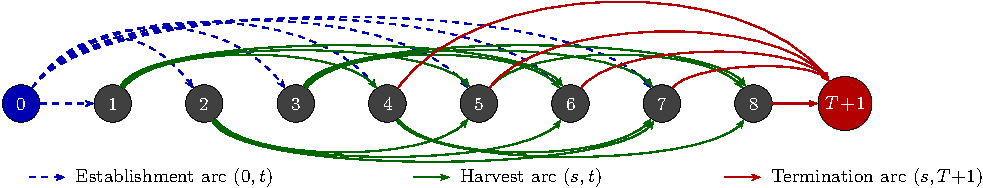
\includegraphics[width=\textwidth]{figures/fig-set-S-tikz-1} 

}

\caption{Network structure of set $\mathcal{S}$ for $T=8$, $A_{\min}=3$, $A_{\max}=5$. Dashed blue arcs: establishment arcs $(0,t)$, $t\in\{1,\ldots,T-1\}$. Solid green arcs above: harvest arcs $(s,t)$ with odd $s$; below: harvest arcs with even $s$. Solid red arcs:    termination arcs $(s,T+1)$, $s\in\{A_{\min}+1,\ldots,T\}$.}\label{fig:fig-set-S-tikz}
\end{figure}

\subsection{Decision Variables}\label{decision-variables}

Temporal flow Variables \(z_{ist}\) indicate on which quantity of the area of site \(i\) an an AFS is operated between \((s,t) \in \mathcal{S}\). Depending on the arc type, this implies establishment, harvest, or termination. Selected arcs buiild a network flow over the complete planning horizon from \(t=0\) to \(T^{max}+1\). \autoref{fig:fig-set-S-path} illustrates a simple network flow with establishment of an AFS in period 1 and harvests in periods 5 and 8.

\begin{figure}

{\centering 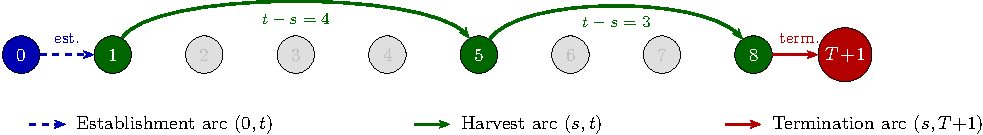
\includegraphics[width=\textwidth]{figures/fig-set-S-path-1} 

}

\caption{Example of a feasible path through the network for $T=8$,$A_{\min}=3$, $A_{\max}=5$: establishment in period~1, harvests in periods~5 and~8, termination at $T+1$.}\label{fig:fig-set-S-path}
\end{figure}

Spatial flow variables \(X_{ijpt}\) and \(X_{jkpp't}\) represent transport of products from AFS sites to storage/pre-treatment facilities and from there to consumers, respectively, while \(S_{jpt}\) captures end-of-period inventory at facility \(j\). \autoref{tab:tab-notation-milp} summarises all sets, decision variables, and parameters used in the MILP formulation, while \(\eta_{pa}\) refers to \eqref{eq:yield}.

\begin{table}[!h]
\centering
\caption{\label{tab:tab-notation-milp}Notation for the MILP model.}
\centering
\resizebox{\ifdim\width>\linewidth\linewidth\else\width\fi}{!}{
\fontsize{8}{10}\selectfont
\begin{tabular}[t]{>{\raggedright\arraybackslash}p{5cm}>{\raggedright\arraybackslash}p{9cm}}
\toprule
\addlinespace[0.3em]
\hline
\multicolumn{2}{l}{\textbf{Sets \& Indices}}\\
\hspace{1em}\cellcolor{gray!10}{$i \in \mathcal{I}$} & \cellcolor{gray!10}{Agroforestry sites}\\
\hspace{1em}$j \in \mathcal{J}$ & Storage / pre-treatment facilities\\
\hspace{1em}\cellcolor{gray!10}{$k \in \mathcal{K}$} & \cellcolor{gray!10}{Consumer sites}\\
\hspace{1em}$p \in \mathcal{P}$ & Product types (stem, branches, residues)\\
\hspace{1em}\cellcolor{gray!10}{$(p,p') \in \mathcal{Q}$} & \cellcolor{gray!10}{Admissible product-substitution pairs (quality cascade)}\\
\hspace{1em}$\mathcal{T}=\{1,\dots,T\}$ & Planning periods (years)\\
\hspace{1em}\cellcolor{gray!10}{$\mathcal{T}^{\text{harv}}=\{A^{\min}+1,\dots,T\}$} & \cellcolor{gray!10}{Feasible harvest periods}\\
\hspace{1em}$\mathcal{S}^{\text{est}}=\{(0,t)\mid t\in\{1,\dots,T-A^{\min}\}\}$ & Establishment arcs: dummy source to period $t$\\
\hspace{1em}\cellcolor{gray!10}{\shortstack[l]{$\mathcal{S}^{\text{harv}}=\{(s,t)\mid s,t\in \mathcal{T},$\\$t-s\in\{A^{\min},\dots,A^{\max}\}\}$}} & \cellcolor{gray!10}{Harvest cycles within age-lag bounds}\\
\hspace{1em}\shortstack[l]{$\mathcal{S}^{\text{term}}=\{(s,T+1)\mid$\\$s\in\{A^{\min}+1,\dots,T\}\}$} & Termination arcs to dummy sink $T+1$\\
\hspace{1em}\cellcolor{gray!10}{$\mathcal{S} = \mathcal{S}^{\text{est}} \cup \mathcal{S}^{\text{harv}} \cup\; \mathcal{S}^{\text{term}}$} & \cellcolor{gray!10}{Age-lag arc set (establishment $\cup$ harvest $\cup$ termination)}\\
\addlinespace[0.3em]
\hline
\multicolumn{2}{l}{\textbf{Decision Variables}}\\
\hspace{1em}$z_{ist} \geq 0$ & Area of site $i$ with AFS operation between $s$ and $t$\\
\hspace{1em}\cellcolor{gray!10}{$X_{ijpt}\ge 0$} & \cellcolor{gray!10}{Transport flow (t) of $p$ from site $i$ to facility $j$ in $t$}\\
\hspace{1em}$X_{jkpp't}\ge 0$ & Flow of $p$ from facility $j$ to consumer $k$ satisfying demand $p'$ in $t$\\
\hspace{1em}\cellcolor{gray!10}{$S_{jpt}\ge 0$} & \cellcolor{gray!10}{Inventory (t) of product $p$ at facility $j$ end of period $t$}\\
\addlinespace[0.3em]
\hline
\multicolumn{2}{l}{\textbf{Parameters}}\\
\hspace{1em}$T$ & Length of planning horizon (years)\\
\hspace{1em}\cellcolor{gray!10}{$A^{\min}$, $A^{\max}$} & \cellcolor{gray!10}{Minimum / maximum stand age at harvest (years)}\\
\hspace{1em}$\text{AREA}_i$ & Area of site $i$ (ha)\\
\hspace{1em}\cellcolor{gray!10}{$\eta_{pa}$} & \cellcolor{gray!10}{Yield coefficient (t/ha) of fraction $p$ at stand age $a$, derived from \eqref{eq:yield}}\\
\hspace{1em}$R_{kp}$ & Revenue (\euro/t) for product $p$ at consumer $k$\\
\hspace{1em}\cellcolor{gray!10}{$C^{\text{est}}_i$} & \cellcolor{gray!10}{Establishment cost (\euro/ha) at site $i$}\\
\hspace{1em}$C^{\text{opp}}_i$ & Annual opportunity cost (\euro/ha) at site $i$\\
\hspace{1em}\cellcolor{gray!10}{$C^{\text{harv}}_i$} & \cellcolor{gray!10}{Harvest \& refitting cost (\euro/ha) at site $i$}\\
\hspace{1em}$c^{\text{tr-raw}}$ & Transport cost rate (\euro/t\,km) for raw biomass\\
\hspace{1em}\cellcolor{gray!10}{$c^{\text{tr-pre}}$} & \cellcolor{gray!10}{Transport cost rate (\euro/t\,km) for pre-treated biomass}\\
\hspace{1em}$c^{\text{stor}}_j$ & Storage holding cost (\euro/t) at facility $j$\\
\hspace{1em}\cellcolor{gray!10}{$d_{ij}$, $d_{jk}$} & \cellcolor{gray!10}{Distance (km) between nodes}\\
\hspace{1em}$\text{CAP}^{\text{stor}}_j/\text{CAP}^{\text{proc}}_j$ & Storage and processing capacity (t) at facility $j$\\
\hspace{1em}\cellcolor{gray!10}{$D^{\max}_{kpt}$} & \cellcolor{gray!10}{Maximum demand (t) of fraction $p$ at consumer $k$ in period $t$}\\
\bottomrule
\end{tabular}}
\end{table}

\subsection{Objective Function}\label{objective-function}

As discussed in Section \ref{sec:lit-afs}, the economic attractiveness of AFS supply chains is modelled from a global perspective taking into account all processes, activities, and participants involved in finally serving customer markets with AFS-based feedstocks. Therefore, revenues for the different biomass fractions and are weighed against costs occurring at all value-adding stages of the supply chains. Revenues created by selling AFS-based feedstocks to different industrial consumers are counterweighted by establishment, opportunity, harvest, transport, and storage costs of landowners, agricultural firms as well as biomass logistics companies. The model therefore maximizes total profit of all participants in the AFS supply chain over the planning horizon as follows:
\begin{align}
\max\; Z \;=\;&
  \sum_{k \in \mathcal{K}}\sum_{p \in \mathcal{P}} R_{kp} \cdot \sum_{j \in \mathcal{J}, }\sum_{(p',p) \in \mathcal{Q}} \sum_{t \in \mathcal{T}}  X_{jkp'pt}  \label{eq:obj-revenue} \\
&- \sum_{i \in \mathcal{I}} c^{{est}}_i \cdot \sum_{(0,t) \in \mathcal{S}^{{est}}} z_{i0t} \notag \\
% &- \sum_{i \in \Ic} c^{{opp}}_i \cdot \left(\sum_{(s,T+1) \in \Sc^{term}} (s+1) \cdot z_{is(T+1)}  -  \sum_{(0,t) \in \Sc^{{est}}}  t \cdot z_{i0t} \right) \notag \\ 
&- \sum_{i \in \mathcal{I}} (c^{main}_{i} + c^{{opp}}_i) \cdot (t-s) \cdot \sum_{(s,t) \in \mathcal{S}^{{harv}}} z_{ist} \notag \\
&- \sum_{i \in \mathcal{I}} c^{{harv}}_i  \cdot \sum_{(s,t) \in \mathcal{S}^{{harv}}} z_{ist} \notag \\
&- \sum_{i \in \mathcal{I}}\sum_{j \in \mathcal{J}}\sum_{p \in \mathcal{P}}\sum_{t \in \mathcal{T}} c^{\text{tr-raw}}_p \cdot d_{ij} \cdot X_{ijpt} \notag \\
&- \sum_{j \in \mathcal{J}}\sum_{k \in \mathcal{K}}\sum_{(p,p') \in \mathcal{Q}} \sum_{t \in \mathcal{T}} c^{\text{tr-pre}}_{p'} \cdot d_{jk} \cdot X_{jkpp't} \notag \\
&- \sum_{j \in \mathcal{J}}\sum_{p \in \mathcal{P}}\sum_{t \in \mathcal{T}}  c^{{stor}}_j \cdot S_{jpt}  \notag
\end{align}

Here, \(R_{kp}\) are product- and consumer-specific revenues for each ton of biomass fraction (\euro{}/t). The opportunity cost term penalises the land use when AFS are established. Thereby, \(c^{{opp}}_i\) can be negative or positive depending on the site-specific conditions. It comprises effect of lost field crop revenues due to AFS as well as higher yields of remaining field crop areas e.g.~due to wind and water erosion protection by AFS. While the assessment of lost field crop revenues is usually well predictable, the economic evaluation of positive ecological effects of AFS (e.g.~on neighboring crop yields) is more difficult. Thus, \(c^{{opp}}_i\) can also contain regulatory subsidies to support establishing and maintaining AFS. Transport cost terms mirror the two-stage flow structure of the AFS supply chain with differentiated rates for raw and pre-treated biomass depending on the biomass type. Cost rates differ because as e.g.~the density and water content of the shipped biomass types differ or because specialized equipment (e.g.~for log transports) is used {[}REFERENCES{]}. Moreover, site-specific establishment cost for planting the AFS trees is considered, next to yearly maintenance and harvesting costs. All these costs scale with the size of a site (\(AREA_i\)) measured in hectar. Maintenance cost comprise e.g.~costs for trimming, replanting, and pruning unnecessary shoots. Storage costs are considered if biomass types are stored for more than a year. Storage cost rate \(c^{{stor}}_j\) measures the costs for storing a ton of biomass for one year and comprises direct storage cost (e.g.~for storage site maintenance) as well as opportunity cost due to potential material losses and capital commitment. Biomass types harvested and consumed in the same year incur no storage cost, as usually AFS are harvested at the beginning of a year. Harvested biomass has to dry during spring and summer such that the biomass can be used in autumn or winter the same year. As under-year drying is necessary for some industrial applications and beneficial for transport economics, drying storage in the year of harvest is not associated with additional cost in this study.

\subsection{Constraints}\label{constraints}

Constraints \eqref{eq:C1} limits the area dedicated to AFS operations to the maximum size of site \(i\). Constraints \eqref{eq:C2} enforce flow conservation in each period. If AFS systems of size \(z_{ist}\) are established or harvested in period \(t \in \mathcal{T}\), there needs to be a succeeding activity (harvest or termination) of this area. This way, \eqref{eq:C2} guarantee valid (possibly empty) AFS activity over the complete time horizon for each site. Constraints \eqref{eq:C3} links the harvest-cycle variables \(z_{ist}\) to physical yield quantities \(\eta^{fw}_{p(t-s)}\) for age \(t-s\), which are pre-computed using \eqref{eq:gomp-stand}--\eqref{eq:yield} scaled by moisture content \(\omega\). Thus, we assume constant yields per hectar for each site \(i\). Note that this simplification can be dropped and site-specific yields \(\eta^{fw}_{ip(t-s)}\) could be introduced without increasing numerical complexity of the AFS-SCD . Constraints \eqref{eq:C5} link harvest quantities to transport flows and ensure inventory balance at each facility. Thereby, harvest quantities can be smaller than available AFS biomass allowing partial harvesting. Constraints \eqref{eq:C6}--\eqref{eq:C7} enforce storage and processing capacity limits at each facility \(j\). Constraints \eqref{eq:C8} implement product usage at multiple consumption sites \(k\). Thereby, \((p',p) \in \mathcal{Q}\) defines a product mapping allowing high-quality product \(p'\) (e.g.~stems) satisfying demand of a lower-quality products \(p\) up to maximum demand \(D^{\max}_{kpt}\).

\begin{align}
  \sum_{(0,t) \in \mathcal{S}^{{est}}} z_{i0t} &\leq AREA_i && \forall\; i \in \mathcal{I}\label{eq:C1} \\[1pt]
  %
  \sum_{(s,t) \in \mathcal{S}} z_{ist} &= \sum_{(t,u) \in \mathcal{S}} z_{itu} && \forall\; i \in \mathcal{I},\; t \in \mathcal{T}\label{eq:C2} \\[1pt]
  %
  \sum_{j \in \mathcal{J}} X_{ijpt}    &\leq \sum_{(s,t) \in \mathcal{S}^{{harv}}} \eta^{fw}_{p(t-s)} \cdot z_{ist} && \forall\; i \in \mathcal{I},\; p \in \mathcal{P},\; t \in \mathcal{T}^{{harv}}     \label{eq:C3} \\[1pt]
  %
  S_{jpt}    = S_{jp,t-1} + &\sum_{i \in \mathcal{I}} X_{ijpt} - \sum_{k \in \mathcal{K},\,(p,p') \in \mathcal{Q}}  X_{jkpp't}   && \forall\; j \in \mathcal{J},\; p \in \mathcal{P},\; t \in \mathcal{T}^{harv}  \label{eq:C5} \\[1pt]
  %
  \sum_{p \in \mathcal{P}} S_{jpt}    &\leq \text{CAP}^{{stor}}_j    && \forall\; j \in \mathcal{J},\; t \in \mathcal{T}\label{eq:C6} \\[1pt]
  %
  \sum_{i \in \mathcal{I},\, p \in \mathcal{P}} X_{ijpt}  &\leq \text{CAP}^{{proc}}_j && \forall\; j \in \mathcal{J},\; t \in \mathcal{T}^{harv} \label{eq:C7} \\[1pt]
  %
  \sum_{j \in \mathcal{J},\,(p',p) \in \mathcal{Q}} X_{jkp'pt} &\leq D^{\max}_{kpt} && \forall\; k \in \mathcal{K},\; p \in \mathcal{P},\; t \in \mathcal{T}^{harv}     \label{eq:C8} \\[1pt]
  %
  z_{ist},\;X_{ijpt},\; &X_{jkp'pt},\; S_{jpt} \geq 0 && \forall\; i,j,k,p,p',t     \label{eq:D2}
  %
\end{align}

In summary, AFS-SCD constitutes are large-scaled LP which allows to decide on which fraction of a site, AFS are established and how the AFS operations are scheduled in a multi-year planning horizon. The AFS-SCD takes a supply chain perspective and maximizes total profit of all actors involved in these processes. Thus, it does not explain how the profits are split e.g.~between farmers, AFS service providers and logistics service providers. The continuous modelling of AFS areas in \(z_{ist}\) leads to a comparatively easy to solve problem. On the other side, it is unclear which part of a site's total area is chosen for AFS operations if \(z_{ist} < AREA_i\), which holds for establishment as well as harvesting and termination.

\section{Case Study}\label{sec-casestudy}

The AFS-SCD is intended to support the design of regional agroforestry biomass supply chains fostering regional bioeconomy clusters thereby connecting multiple industrial sectors. The proposed AFS-SCD model is instantiated on a real-world biomass supply chain case study located in the tri-state region of Saxony-Anhalt, northern Thuringia, and northern Saxony, Germany. This region is characterized by a high density of agricultural land usage as well as cluster of paper and wood as well as chemical industry. The regional chemical industry relies on fossil ressources so fa, but is under substantial transformative pressure which led to investments in sustainable production processes requiring sustainable regional bio-based feedstocks. \autoref{fig:fig-supply-chain-network} shows agricultural production sites along with the set of potential wood-processing hubs, and the regional users of AFS biomasses from chemical, paper and wood processing industry as well as the energy sector.

\begin{figure}

{\centering 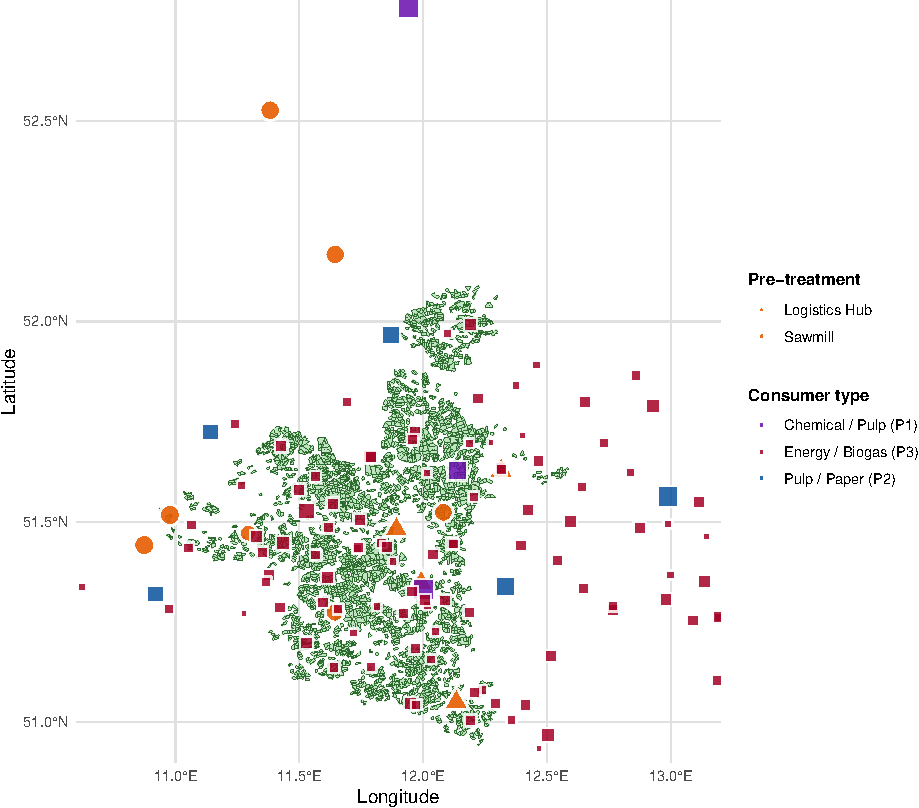
\includegraphics[width=\textwidth]{figures/fig-supply-chain-network-1} 

}

\caption{AFS supply chain network in Saxony-Anhalt. Grey lines: German federal state boundaries. Blue lines: major rivers. Coloured polygons: potential AFS parcels grouped by site (colours encode cluster membership; no legend). Orange symbols: pre-treatment facilities (circle = sawmill, triangle = logistics hub, size proportional to processing capacity). Coloured squares: consumer sites (violet: P1 chemical/pulp, blue: P2 pulp/paper, red: P3 energy/biogas, size proportional to total demand).}\label{fig:fig-supply-chain-network}
\end{figure}

The supply chain comprises 2239 agricultural production parcels which are grouped into \(|\mathcal{I}|=\) 145 potential AFS production sites. Clustering is based on geographical distances between parcel centroid using a k-means approach in order to reduce problem size. For distance calculations, for each site a centroid is calculated. Pre-treatment and intermediate storage facilities \(\mathcal{J}\) are located on existing wood processing facilities as well as potential new log or wood chip yards. All harvested biomass quantities at AFS sites are transported to logistics hubs first. At the hubs sorting and transshipment processes take place before biomass types are forwarded to the consumer facilities. Storing and transshipment capacities at the hibs are assumed to be constant in time and universally set to \ensuremath{4.0909\times 10^{4}} kt per year. Finally, \(|\mathcal{K}|=\) 28 consumer sites are included. Each consumer site belongs to an existing facility from chemical, paper/wood processing industry, or the energy sector. Distances between the facilities \(d_{ij}\) and \(d_{jk}\) are calculated as road distances between the facilities' coordinates. For each consumer facility, an yearly upper demand capacity for each of the three distinguished biomass product types are given along with consumer-specific prices. The following biomass types are distinguished:

\begin{itemize}
\item
  \textbf{P1: stem wood -- chemical/paper grade}: long-fibre wood chips from stems suitable for conversion in a local biorefinery and paper factory. In total, a yearly demand of 620 kt and an average prices of 45 € is assumed.
\item
  \textbf{P2: branch wood -- sawmill/pulp grade}: medium/short-fibre wood chips from larger branches suitable for mechanical processing in sawmills and lower-grade pulping. Demand is distributed across 6 smaller facilities and accumulates to 410 kt/year. Gate prices range from 28-38 €/t.
\item
  \textbf{P3: residue -- energy grade}: residual wood fractions (chips, bark, off-cuts) used for heat and electricity generation or lower-grade pellet production. Demand is accumulates among 24 consumers to 132 kt/year. Gate prices range from 18-24 €/t.
\end{itemize}

\autoref{tab:tab-consumers} in the appendix summarizes the consumer-specific demand data. It is assumed that the biomass product types show a quality cascade which means that the demand of pulp grade (P2) can also be satisfied by chemical/paper grade biomass (P1). Likewise, energy grade demand (P3) can be satisfied by all biomass types. Note that constant demands over the planning horizon are assumed, although an increasing biomass demand can be expected due to the green transition in those industries. From this perspective, a rather conservative market demand scenario is assumed.

Growth model introduced in \autoref{sec:lit-growth} is used to model biomass quantities depending on age and the area dedicated to AFS. The growth model is parameterized for poplar clones at central European conditions as introduced above with a planting density of \(N=400\) trees per hectar. If AFS are established, they have to be harvested within \(A^{\\min}=\) 3 to \(A^{\\max}=\) 20 years allowing a wide range of potential harvesting strategies between short-rotation and long-rotation AFS. As the total planning horizon is \(|\mathcal{T}|=\) 40 years multiple harvesting cycles can be established. The sites do not differ with respect to growth conditions as the climatic and soil quality variation within the comparatively small region is rather limited. However, the sites differ with respect to size (given in hectar) and opportunity cost rates (given in € per hectar and year). Site-specific opportunity cost rates \(c^{opp}_i\) is normally distributed with mean 521 and standard deviation 391. For most sites, substantial opportunity costs are assumed reflecting the loss in field-crop revenue, risk premiums of landowners as well as higher costs for field crop maintenance. The 145 sites with negative opportunity cost rates reflect sites where AFS lead to an increase in field crop productivity on the remaining field area. The variation in opportunity cost rates to study the effect of opportunity cost on site selection for AFS and gives valuable insights particularly for communication with farmers and politics. Subsidies for establishing AFS are one of the core instruments to foster AFS. The height and effectiveness of those subsidies, however, is controversially disputed. Remaining cost parameters are universally set for all sites and comprise maintenance cost rates \(c^{main}_i\) (€ per year and hectar), establishment cost \(c^{est}_i\) (€ per hectar) and harvesting cost \(c^{harv}_i\) (€ per hectar). Likewise, transport cost rates for harvested biomasses \(c^{tr-raw}_p\) and pre-treated/sorted biomasses \(c^{tr-raw}_{p'}\) are set universally. All scalar parameters are shown in \autoref{tab:tab-milp-params}.

\begin{table}[!h]
\centering
\caption{\label{tab:tab-milp-params}Parameter values for the AFS-SCD case study. Transport costs refer to road distance}
\centering
\fontsize{8}{10}\selectfont
\begin{tabular}[t]{llrl}
\toprule
Parameter & Description & Base-case value & Unit\\
\midrule
\addlinespace[0.3em]
\multicolumn{4}{l}{\textbf{Index sets}}\\
\hspace{1em}\cellcolor{gray!10}{$|\mathcal{T}|$} & \cellcolor{gray!10}{Planning periods} & \cellcolor{gray!10}{40} & \cellcolor{gray!10}{yr}\\
\hspace{1em}$|\mathcal{I}|$ & Sites & 145 & –\\
\hspace{1em}\cellcolor{gray!10}{$|\mathcal{J}|$} & \cellcolor{gray!10}{Pre-treatment / storage nodes} & \cellcolor{gray!10}{11} & \cellcolor{gray!10}{–}\\
\hspace{1em}$|\mathcal{K}|$ & Consumers & 28 & –\\
\hspace{1em}\cellcolor{gray!10}{$|\mathcal{P}|$} & \cellcolor{gray!10}{Product grades} & \cellcolor{gray!10}{3} & \cellcolor{gray!10}{–}\\
\addlinespace[0.3em]
\multicolumn{4}{l}{\textbf{Biomass dynamics}}\\
\hspace{1em}$A^{\min}$ & Minimum harvest age (years) & 3 & yr\\
\hspace{1em}\cellcolor{gray!10}{$A^{\max}$} & \cellcolor{gray!10}{Maximum stand age (years)} & \cellcolor{gray!10}{20} & \cellcolor{gray!10}{yr}\\
\addlinespace[0.3em]
\multicolumn{4}{l}{\textbf{Cost parameters}}\\
\hspace{1em}$c^{tr\text{-}raw}$ & Raw transport cost & 0.08 & € t$^{-1}$ km$^{-1}$\\
\hspace{1em}\cellcolor{gray!10}{$c^{tr\text{-}pre}$} & \cellcolor{gray!10}{Pre-processed transport cost} & \cellcolor{gray!10}{0.06} & \cellcolor{gray!10}{€ t$^{-1}$ km$^{-1}$}\\
\hspace{1em}$c^{est}_i$ & Establishment cost rate & 2500 & € ha$^{-1}$ yr$^{-1}$\\
\hspace{1em}\cellcolor{gray!10}{$c^{harv}_i$} & \cellcolor{gray!10}{harvest cost rate} & \cellcolor{gray!10}{150} & \cellcolor{gray!10}{€ ha$^{-1}$ yr$^{-1}$}\\
\hspace{1em}$c^{main}_i$ & Maintenance cost rate & 10 & € ha$^{-1}$ yr$^{-1}$\\
\hspace{1em}\cellcolor{gray!10}{$c_i^{opp}$} & \cellcolor{gray!10}{aver. opportunity cost} & \cellcolor{gray!10}{521} & \cellcolor{gray!10}{€ ha$^{-1}$ yr$^{-1}$}\\
\addlinespace[0.3em]
\multicolumn{4}{l}{\textbf{Revenue parameters}}\\
\hspace{1em}$R_{P1}$ & Mean gate price P1 & 45 & € t$^{-1}$\\
\hspace{1em}\cellcolor{gray!10}{$R_{P2}$} & \cellcolor{gray!10}{Mean gate price P2} & \cellcolor{gray!10}{33} & \cellcolor{gray!10}{€ t$^{-1}$}\\
\hspace{1em}$R_{P3}$ & Mean gate price P3 & 21 & € t$^{-1}$\\
\bottomrule
\end{tabular}
\end{table}

\subsection{Optimization results}\label{optimization-results}

The AFS-SCD model is solved for the instance data described above with Gurobi. The model selects a subset of sites for AFS establishment and identifies the optimal harvest schedules, intermediate facility utilisation, and product allocation across the planning horizon.

\autoref{fig:fig-results-sc-map} shows the spatial configuration of the profit-optimal supply chain.

\begin{figure}

{\centering 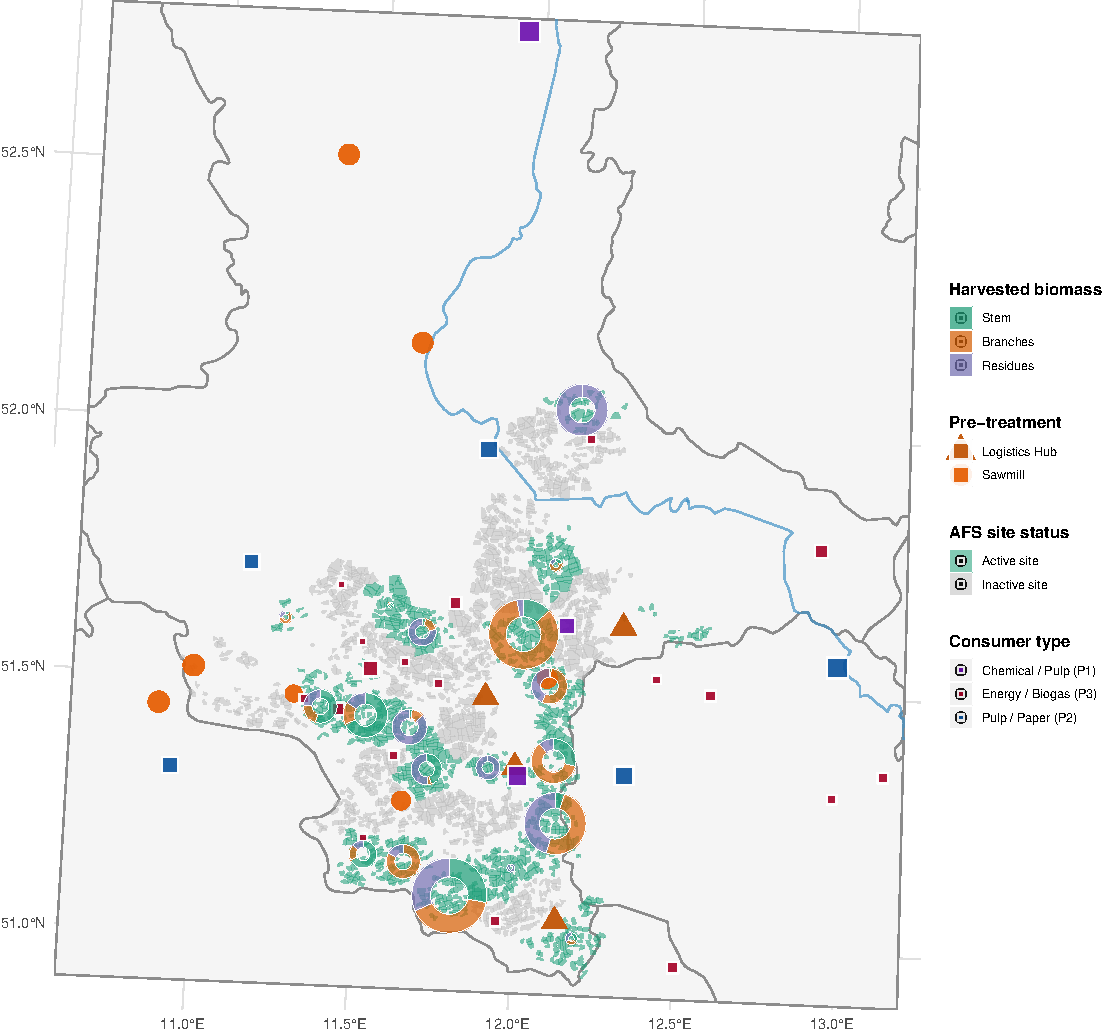
\includegraphics[width=.9\textwidth]{figures/fig-results-sc-map-1} 

}

\caption{Site selection and biomass production in optimal supply chain configuration. Green polygons: active sites with biomass harvest; grey polygons: non-selected sites. Pie charts at active sites show the product mix of harvested biomass, scaled by total harvested volume.}\label{fig:fig-results-sc-map}
\end{figure}

In total, on 38 sites AFS are established which corresponds to about 26 \% of all sites and 24 \% of the total farm area. Over the planning horizon, \ensuremath{2.6368\times 10^{4}} kt of AFS biomasses are produced on these sites which suffices to satisfy 57 \% of total demand. \autoref{fig:fig-results-product-mix} shows the harvested biomasses over time along with total demand of all consumer sites.

\begin{figure}

{\centering 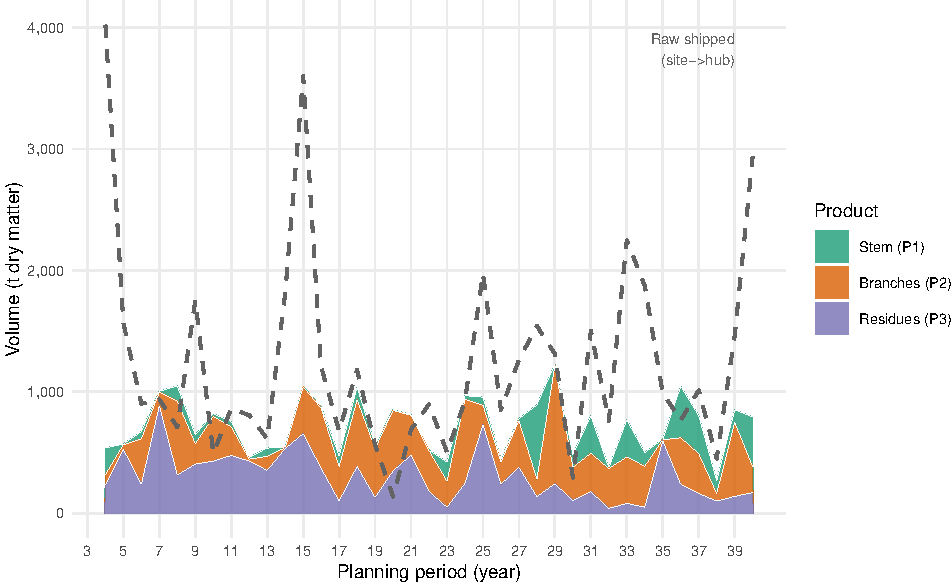
\includegraphics[width=\textwidth]{figures/fig-results-product-mix-1} 

}

\caption{Total biomass delivered to consumers by product type over the planning horizon. Stacked areas show period-level volumes of stem (P1), branches (P2), and residues (P3) flowing from storage hubs to all consumers. Dashed line: total harvested raw biomass shipped from sites to hubs.}\label{fig:fig-results-product-mix}
\end{figure}

During the first 10 years no AFS biomasses are harvested as trees of established AFS in first years grow up to a certain size before first harvest. Thus, about 25\% of consumers' total biomass demand cannot be satisfied due to this grow-up period. Afterwards, a cyclical pattern appears with a harvesting peak around year 20 and a breakdown in year 28 before plateau is reached from year 35-40. Thereby, the harvesting quantities of stems and branches show a similar pattern while quantities of harvested energy grade biomass are rather stable and close to the demand limit over the planning horizon. Thus, rather long-rotation AFS are established as \autoref{fig:fig-results-harvest-cycle-dist} confirms showing the histogram of harvesting ages across all sites.

\begin{figure}

{\centering 
\includegraphics[width=\textwidth]{figures/fig-results-harvest-cycle-dist-1} 

}

\caption{Distribution of harvesting cycle lengths at active agroforestry sites. Each bar represents the number of individual harvest events (over all periods and active sites) whose cycle length (stand age at harvest, i.e. $t - s$) falls in that year bin.}\label{fig:fig-results-harvest-cycle-dist}
\end{figure}

The histogram illustrates that majority of harvest events occur at stand ages between 14--18 years, indicating that long-rotation AFS seem to be more profitable in this setting. Short-rotation cycles (\textless10 years) occur only in marginal frequencies. This optimal rotation length might be caused either due to the limited demand of energy-grade biomass or the price gaps between biomass types or a combination of effects. The quantity of energy-grade biomass created in long-rotation AFS suffices to cover total energy-grade biomass demand almost completely. Rotation length is focused on production of chemical-grade biomass where highest prices are assumed. Focusing on chemical industry supply requires a production of trees with a comparatively large stems. This strategy maximizes revenue, but in the same time increases opportunity costs as wood harvests appear in larger time intervals. \autoref{fig:fig-results-cost-profit-breakdown} presents the aggregate cost--profit waterfall over all periods and actors.

\begin{figure}

{\centering 
\includegraphics[width=\textwidth]{figures/fig-results-cost-profit-breakdown-1} 

}

\caption{Total cost–profit breakdown across all actors and years. The left panel (waterfall) decomposes the objective value into revenue and individual cost categories; the right panel shows the period-level trajectory of revenues and stacked costs.}\label{fig:fig-results-cost-profit-breakdown}
\end{figure}

It appears that revenue is dominated by selling chemical-grade biomass and dominating cost component are opportunity cost although active sites are those sites with a comparatively small opportunity cost rate. Next to opportunity cost, establishment and transport costs are the most relevant cost drivers. Analyzing total cashflow over time shows that break-even is reached after about 20 years, i.e.~after the first large-scale harvest occurred. Afterwards, cashflow is continuously increasing indicating that establishing AFS is a strategic change in agricultural practice and pays only if this strategy is implemented and maintained over a comparatively long time spans. This underpins the importance of strategic buying contracts with industrial partners in order to reduce revenue risks of farmers when producing AFS biomass.

Although profitability of the total AFS suply chain is given for the case study data, profitability of AFS operations on site-level are more heterogeneous. \autoref{fig:fig-results-site-breakdown} shows revenues and costs split by component and normalized to AFS size and active years of AFS.

\begin{figure}

{\centering 
\includegraphics[width=\textwidth]{figures/fig-results-site-breakdown-1} 

}

\caption{Revenues, costs and net profit for sites with AFS operations split by type and expressed in € per hectare per year of AFS operation.}\label{fig:fig-results-site-breakdown}
\end{figure}

It appears that net profitability of AFS ranges between 282 and 6 € per hectare and active year. Note that this value constitutes additional profit after subtracting operational cost as well as imputed opportunity cost of lost profit from field crop. I.e., for calculating the realized net margin, opportunity can be added such that realized yearly net profit ranges between 473 and 210 € per hectare. Still, relative net profit is comparatively low compared to ordinary agricultural practices with profitable field crops (like winter wheat). The revenue splits of active sites indicates that at some sites medium-grade and low-grade biomass types contribute substantially or even solely to total revenue (see e.g.~site 12, 135, 145, and 112). This indicates that site-specific AFS strategies might differ from the overall supply chain strategy. In other words, there seem to be strategic niches w.r.t. the consumer segments to be supplied. This might also be reflected in the rotation length and, although not discussed here, the selection of trees and clones for the AFS. Moreover, profitability of AFS sites seems to depend on various factors like local opportunity costs as well as closeness to consumers. \autoref{fig:fig-results-site-scatter} shows net margins and opportunity cost rates of sites with active AFS.

\begin{figure}

{\centering 
\includegraphics[width=\textwidth]{figures/fig-results-site-scatter-1} 

}

\caption{Scatterplot of opportunity cost rate and net margin (both in € per ha and year) for each site with active AFS. Size of AFS reflected in point size.}\label{fig:fig-results-site-scatter}
\end{figure}

As expected net margins of AFS depend heavily on a site's opportunity cost rate showing a clear negative trend. Moreover, it appears that AFS sizes vary quite heavily between 86 and 2794 hectare. Probably very small sites won't operate efficiently because cost for establishment, harvesting, and maintenance are assumed to scale with size, but are rather fixed below a certain critical threshold.

\section{Conclusion}\label{conclusion}

This paper has developed and applied the AFS-SCD model, a MILP
formulation for the integrated design and operation of agroforestry
biomass supply chains. The model endogenises stand age dynamics through
binary arc-based age-lag variables, couples component-specific Gompertz
yield coefficients for stem, branch, and residue fractions with
multi-echelon logistics decisions, and embeds a product quality cascade
that allocates biomass grades to chemical, pulp, and energy markets
within a unified optimisation framework. The formulation is, to the best
of our knowledge, the first supply chain model to simultaneously
optimise AFS establishment timing, consecutive harvest scheduling under
rotation-age constraints, and product-grade allocation across spatially
heterogeneous consumer markets.

The case study for the Saxony-Anhalt tri-state region demonstrates the
practical relevance of the approach. The optimal supply chain
concentrates AFS establishments in the Elbe and Saale floodplains,
where high biomass productivity and proximity to large pulp mills create
the most favourable economics. The sensitivity analysis confirms that
profitability depends primarily on achievable gate prices for
high-quality (P1) biomass grades: scenarios combining reduced revenue
with high opportunity costs yield negative net profits, whereas
scenarios with full or elevated prices remain viable under cost pressure.
Opportunity cost is the dominant site-level discriminator, with parcels
exceeding approximately 300 \euro~ha\(^{-1}\) yr\(^{-1}\) rarely selected
in the optimal solution. These findings underscore the importance of
product cascading as a strategic lever for AFS viability: maximising
the share of stem biomass directed to high-value chemical and pulp
applications substantially improves profitability compared to
energy-only offtake strategies.

Methodologically, the AFS-SCD model bridges the gap between stand-level
growth modelling and regional supply chain optimisation identified in
the literature (Lamers et al., 2011; Zahraee et al., 2020).
The age-lag constraint structure generalises to other perennial biomass
crops with periodic coppice cycles, such as willow or black locust, and
to long-rotation silvoarable systems in which rotation length is a
strategic variable. The model is extensible to stochastic settings by
replacing deterministic yield coefficients with scenario-weighted
counterparts or by incorporating robust optimisation over yield
uncertainty intervals (Sharma et al., 2013).

Several limitations point to directions for future research. First,
consumer demand is treated as exogenous and time-invariant; endogenising
demand responses to biomass price changes would require a
partial-equilibrium extension. Second, the case study uses a single
allometric scenario calibrated to Central European poplar; propagating
Gompertz parameter uncertainty through to supply chain outcomes would
strengthen the robustness analysis. Third, environmental co-benefits of
AFS --- including carbon sequestration, nitrate leaching reduction, and
biodiversity enhancement --- are not monetised in the current objective.
Integrating life cycle assessment indicators as additional objectives
or constraints would support a more comprehensive sustainability
evaluation, consistent with the cleaner production framing of this work.

\section{Appendix}\label{appendix}

\begin{figure}

{\centering \includegraphics[width=\textwidth]{figures/growth-asymptote-functions-1} 

}

\caption{Tree-level and stand-level Gompertz asymptote functions $A_{tree}(N)$ and $A(N)$ for advanteguous ($N=4$, $\beta=-0.3$) and disadvantageous ($N=6.5$, $\beta=-0.5$) site conditions.}\label{fig:growth-asymptote-functions}
\end{figure}

\begin{table}[!h]
\centering
\caption{\label{tab:tab-notation-growth}Notation for the biomass growth and harvest yield models.}
\centering
\resizebox{\ifdim\width>\linewidth\linewidth\else\width\fi}{!}{
\fontsize{8}{10}\selectfont
\begin{tabular}[t]{>{\raggedright\arraybackslash}p{3.2cm}>{\raggedright\arraybackslash}p{10.8cm}}
\toprule
Symbol & Description\\
\midrule
\cellcolor{gray!10}{$M(t)$} & \cellcolor{gray!10}{Total above- and belowground dry biomass per ha of AFS (t\,DM\,ha$^{-1}$) at stand age $t$}\\
$A(N)$ & Stand-level Gompertz asymptote (t\,DM\,ha$^{-1}$); density- and site-dependent\\
\cellcolor{gray!10}{$k$} & \cellcolor{gray!10}{Gompertz growth-rate coefficient}\\
$t_0$ & Inflection age of stand biomass accumulation (years)\\
\cellcolor{gray!10}{$N$} & \cellcolor{gray!10}{Stand density (trees\,ha$^{-1}$)}\\
\addlinespace
$C_{\mathrm{site}}$ & Site-quality constant (kg\,ha$^{\beta-1}$); conservative: 4\,475, good site: 6\,471\\
\cellcolor{gray!10}{$\beta$} & \cellcolor{gray!10}{Competition-density exponent; fitted $\hat{\beta}=0.380$}\\
$f_p(t)$ & asymtotic fraction of AGB attributed to compartment $p \in \{s,b,r\}$ at age $t$\\
\cellcolor{gray!10}{$q_p(t)$} & \cellcolor{gray!10}{Merchantable fraction of compartment $p$ biomass at age $t$ (logistic)}\\
$r_p$ & Logistic growth rate for merchantability of compartment $p$\\
\addlinespace
\cellcolor{gray!10}{$t_{50,p}$} & \cellcolor{gray!10}{Age at which 50\% of compartment $p$ biomass is merchantable (yr)}\\
$\eta_p(t)$ & Merchantable dry biomass of compartment $p$ per ha at harvest age $t$ (t\,DM\,ha$^{-1}$)\\
\cellcolor{gray!10}{$\omega$} & \cellcolor{gray!10}{Moisture content at felling (mass fraction); $\omega = 0.55$}\\
\bottomrule
\end{tabular}}
\end{table}

\begin{table}[!h]
\centering
\caption{\label{tab:tab-consumers}Consumer demand quantities and gate prices by product grade. P1: chemical/pulp; P2: sawlog/pulpwood; P3: energy/pellets. Demands in kt wood input per year; prices in €/t wood input at the factory gate.}
\centering
\resizebox{\ifdim\width>\linewidth\linewidth\else\width\fi}{!}{
\fontsize{8}{10}\selectfont
\begin{tabular}[t]{lrrrrrr}
\toprule
\multicolumn{1}{c}{ } & \multicolumn{3}{c}{Annual demand} & \multicolumn{3}{c}{Gate price} \\
\cmidrule(l{3pt}r{3pt}){2-4} \cmidrule(l{3pt}r{3pt}){5-7}
Consumer & P1 (kt/yr) & P2 (kt/yr) & P3 (kt/yr) & P1 (€/t) & P2 (€/t) & P3 (€/t)\\
\midrule
\cellcolor{gray!10}{consumer  1} & \cellcolor{gray!10}{300.0} & \cellcolor{gray!10}{–} & \cellcolor{gray!10}{–} & \cellcolor{gray!10}{50} & \cellcolor{gray!10}{–} & \cellcolor{gray!10}{–}\\
consumer  2 & 100.0 & – & – & 60 & – & –\\
\cellcolor{gray!10}{consumer  3} & \cellcolor{gray!10}{–} & \cellcolor{gray!10}{300} & \cellcolor{gray!10}{50.0} & \cellcolor{gray!10}{–} & \cellcolor{gray!10}{37.5} & \cellcolor{gray!10}{24}\\
consumer  4 & 200.0 & – & – & 47.5 & – & –\\
\cellcolor{gray!10}{consumer  5} & \cellcolor{gray!10}{–} & \cellcolor{gray!10}{30} & \cellcolor{gray!10}{5.0} & \cellcolor{gray!10}{–} & \cellcolor{gray!10}{35} & \cellcolor{gray!10}{21}\\
\addlinespace
consumer  6 & – & 15 & 5.0 & – & 32.5 & 21\\
\cellcolor{gray!10}{consumer  7} & \cellcolor{gray!10}{–} & \cellcolor{gray!10}{10} & \cellcolor{gray!10}{3.0} & \cellcolor{gray!10}{–} & \cellcolor{gray!10}{30} & \cellcolor{gray!10}{18}\\
consumer  8 & – & 5 & 8.0 & – & 27.5 & 18\\
\cellcolor{gray!10}{consumer  9} & \cellcolor{gray!10}{2.0} & \cellcolor{gray!10}{50} & \cellcolor{gray!10}{20.0} & \cellcolor{gray!10}{40} & \cellcolor{gray!10}{35} & \cellcolor{gray!10}{22.8}\\
consumer  10 & – & – & 1.7 & – & – & 21\\
\addlinespace
\cellcolor{gray!10}{consumer  11} & \cellcolor{gray!10}{–} & \cellcolor{gray!10}{–} & \cellcolor{gray!10}{2.9} & \cellcolor{gray!10}{–} & \cellcolor{gray!10}{–} & \cellcolor{gray!10}{21}\\
consumer  12 & – & – & 2.5 & – & – & 21\\
\cellcolor{gray!10}{consumer  13} & \cellcolor{gray!10}{–} & \cellcolor{gray!10}{–} & \cellcolor{gray!10}{2.3} & \cellcolor{gray!10}{–} & \cellcolor{gray!10}{–} & \cellcolor{gray!10}{21}\\
consumer  14 & – & – & 1.9 & – & – & 21\\
\cellcolor{gray!10}{consumer  15} & \cellcolor{gray!10}{–} & \cellcolor{gray!10}{–} & \cellcolor{gray!10}{2.7} & \cellcolor{gray!10}{–} & \cellcolor{gray!10}{–} & \cellcolor{gray!10}{21}\\
\addlinespace
consumer  16 & – & – & 1.7 & – & – & 21\\
\cellcolor{gray!10}{consumer  17} & \cellcolor{gray!10}{–} & \cellcolor{gray!10}{–} & \cellcolor{gray!10}{1.9} & \cellcolor{gray!10}{–} & \cellcolor{gray!10}{–} & \cellcolor{gray!10}{21}\\
consumer  18 & – & – & 1.6 & – & – & 21\\
\cellcolor{gray!10}{consumer  19} & \cellcolor{gray!10}{–} & \cellcolor{gray!10}{–} & \cellcolor{gray!10}{1.5} & \cellcolor{gray!10}{–} & \cellcolor{gray!10}{–} & \cellcolor{gray!10}{21}\\
consumer  20 & – & – & 1.5 & – & – & 21\\
\addlinespace
\cellcolor{gray!10}{consumer  21} & \cellcolor{gray!10}{–} & \cellcolor{gray!10}{–} & \cellcolor{gray!10}{1.8} & \cellcolor{gray!10}{–} & \cellcolor{gray!10}{–} & \cellcolor{gray!10}{21}\\
consumer  22 & – & – & 3.5 & – & – & 21\\
\cellcolor{gray!10}{consumer  23} & \cellcolor{gray!10}{–} & \cellcolor{gray!10}{–} & \cellcolor{gray!10}{1.6} & \cellcolor{gray!10}{–} & \cellcolor{gray!10}{–} & \cellcolor{gray!10}{21}\\
consumer  24 & – & – & 2.1 & – & – & 21\\
\cellcolor{gray!10}{consumer  25} & \cellcolor{gray!10}{–} & \cellcolor{gray!10}{–} & \cellcolor{gray!10}{4.5} & \cellcolor{gray!10}{–} & \cellcolor{gray!10}{–} & \cellcolor{gray!10}{21}\\
\addlinespace
consumer  26 & – & – & 1.8 & – & – & 21\\
\cellcolor{gray!10}{consumer  27} & \cellcolor{gray!10}{–} & \cellcolor{gray!10}{–} & \cellcolor{gray!10}{3.2} & \cellcolor{gray!10}{–} & \cellcolor{gray!10}{–} & \cellcolor{gray!10}{21}\\
consumer  28 & 18.5 & – & – & 27.5 & – & –\\
\bottomrule
\end{tabular}}
\end{table}

\begin{figure}

{\centering 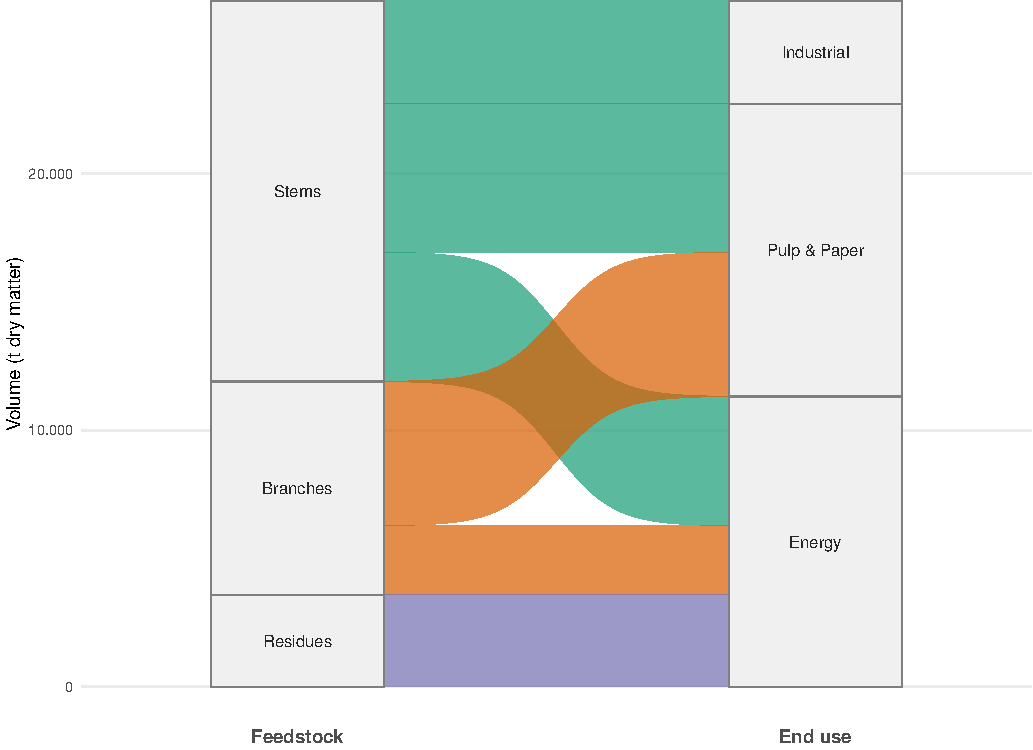
\includegraphics[width=\textwidth]{figures/fig-results-harvest-gantt-1} 

}

\caption{Total production quantity of biomass types and its industrial usage over planning horizon (in tons).}\label{fig:fig-results-harvest-gantt}
\end{figure}

\protect\phantomsection\label{refs}
\begin{CSLReferences}{1}{0}
\bibitem[\citeproctext]{ref-Arabi2019_Microalgae_Biobutanol_SC}
Arabi, M., Yaghoubi, S., \& Tajik, H. (2019). Optimal design of a microalgae-based biofuel supply chain with CO2 reduction and hydrogen production. \emph{Computers \& Chemical Engineering}, \emph{130}, 106530. \url{https://doi.org/10.1016/j.compchemeng.2019.106530}

\bibitem[\citeproctext]{ref-Cambero2014_ForestBSC_Review}
Cambero, C., \& Sowlati, T. (2014). Assessment and optimization of forest biomass supply chains from economic, social and environmental perspectives---a review of literature. \emph{Renewable and Sustainable Energy Reviews}, \emph{36}, 62--73. \url{https://doi.org/10.1016/j.rser.2014.04.041}

\bibitem[\citeproctext]{ref-Civitarese2019_Poplar_Harvest}
Civitarese, V., Acampora, A., Sperandio, G., Assirelli, A., \& Picchio, R. (2019). Production of wood pellets from poplar trees managed as coppices with different harvesting cycles. \emph{Energies}, \emph{12}(15), 2973. \url{https://doi.org/10.3390/en12152973}

\bibitem[\citeproctext]{ref-DeMeyer2015_OPTIMASS}
De Meyer, A., Cattrysse, D., Rasinmäki, J., \& Van Orshoven, J. (2014). Methods to optimise the design and management of biomass-for-bioenergy supply chains: {A} review. \emph{Renewable and Sustainable Energy Reviews}, \emph{31}, 657--670. \url{https://doi.org/10.1016/j.rser.2013.12.036}

\bibitem[\citeproctext]{ref-DeMeyer2016_tOPTIMASS}
De Meyer, A., Cattrysse, D., \& Van Orshoven, J. (2016). A generic mathematical model to optimise strategic and tactical decisions in biomass-based supply chains ({OPTIMASS}). \emph{European Journal of Operational Research}, \emph{249}(1), 293--307. \url{https://doi.org/10.1016/j.ejor.2015.08.003}

\bibitem[\citeproctext]{ref-DEFAF}
Deutscher Fachverband für Agroforstwirtschaft (DeFAF) e.V. (2026). \emph{Annual review of the {Agroforestry Map of Germany} 2025}. \url{https://agroforst-info.de/wp-content/uploads/2026/02/DeFAF-2026-Annual-review-of-the-Agroforestry-Map-of-Germany-2025.pdf}

\bibitem[\citeproctext]{ref-Eksioglu2009_Biorefinery_SC}
Ekşioğlu, S. D., Acharya, A., Leightley, L. E., \& Arora, S. (2009). Analyzing the design and management of biomass-to-biorefinery supply chain. \emph{Computers \& Industrial Engineering}, \emph{57}(4), 1342--1352. \url{https://doi.org/10.1016/j.cie.2009.07.003}

\bibitem[\citeproctext]{ref-Espinoza2017_Biorefinery_SC_review}
Espinoza, V., Bautista, S., Narvaez, P. C., Alfaro, M., \& Camargo, M. (2017). Sustainability assessment to support governmental biodiesel policy in {Colombia}: {A} system dynamics model. \emph{Journal of Cleaner Production}, \emph{141}, 1145--1163. \url{https://doi.org/10.1016/j.jclepro.2016.09.168}

\bibitem[\citeproctext]{ref-Faasch2012_SRC_Economics}
Faasch, R. J., \& Patenaude, G. (2012). The economics of short rotation coppice in {Germany}. \emph{Biomass and Bioenergy}, \emph{45}, 27--40. \url{https://doi.org/10.1016/j.biombioe.2012.04.012}

\bibitem[\citeproctext]{ref-Graves2007_Agroforestry_Economics}
Graves, A. R., Burgess, P. J., Liagre, F., Pisanelli, A., Paris, P., Moreno, G., Bellido, M., Mayus, M., Postma, M., Schindler, B., Mantzanas, K., \& Dupraz, C. (2007). Development and application of bio-economic modelling to compare silvoarable, arable, and forestry systems in three {European} countries. \emph{Ecological Engineering}, \emph{29}(4), 434--449. \url{https://doi.org/10.1016/j.ecoleng.2006.09.018}

\bibitem[\citeproctext]{ref-Grunewald2007_Robinia_AFS}
Grünewald, H., Böcker, R., Schneider, B. U., Bens, O., \& Hüttl, R. F. (2007). Biomass production of black locust ({Robinia pseudoacacia} {L}.) short rotation plantations in {Germany}: Growth and economics of different clones and management practices. \emph{Bioresource Technology}, \emph{98}(2), 281--286. \url{https://doi.org/10.1016/j.biortech.2006.01.004}

\bibitem[\citeproctext]{ref-Hildebrandt2019}
Hildebrandt, J., O'Keeffe, S., Bezama, A., \& Thrän, D. (2019). Revealing the environmental advantages of industrial symbiosis in wood-based bioeconomy networks: An assessment from a life cycle perspective. \emph{Journal of Industrial Ecology}, \emph{23}(4), 808--822. \url{https://doi.org/10.1111/jiec.12818}

\bibitem[\citeproctext]{ref-Huber2018_SRAFS_growth}
Huber, G., Amann, C., Hülsbergen, K.-J., \& Schmid, H. (2018). Yield potential of tree species in organic and conventional short-rotation agroforestry systems in {Southern Germany}. \emph{Heliyon}, \emph{4}(1), e00543. \url{https://doi.org/10.1016/j.heliyon.2018.e00543}

\bibitem[\citeproctext]{ref-Huber2016_Allometric_SRAFS}
Huber, G., Hülsbergen, K.-J., \& Schmid, H. (2016). Allometric equations for above-ground tree-biomass estimation in {Southern German} short-rotation agroforestry systems. \emph{Bioenergy Research}, \emph{9}(3), 955--968. \url{https://doi.org/10.1007/s12155-016-9744-z}

\bibitem[\citeproctext]{ref-Jha2018_Poplar_AFS_Biomass}
Jha, K. K. (2018). Biomass production and carbon balance in two hybrid poplar ({\emph{Populus euramericana}}) plantations raised with and without agriculture in southern {France}. \emph{Journal of Forestry Research}, \emph{29}(6), 1689--1701. \url{https://doi.org/10.1007/s11676-017-0555-3}

\bibitem[\citeproctext]{ref-Shinozaki1961_CD_Effect}
Kira, T., Shinozaki, K., \& Hozumi, K. (1961). The {C-D} rule, its theory and practical uses. ({Intraspecific competition among higher plants. X.}). \emph{Journal of Biology, Osaka City University}, \emph{12}, 69--82.

\bibitem[\citeproctext]{ref-Lamers2015_Feedstock_Design}
Lamers, P., Junginger, M., Hamelinck, C., \& Faaij, A. (2011). Developments in liquid biofuels commodity trade. \emph{Biofuels, Bioproducts and Biorefining}, \emph{5}(4), 403--437. \url{https://doi.org/10.1002/bbb.303}

\bibitem[\citeproctext]{ref-Malladi2018_BSC_Logistics}
Malladi, K. T., \& Sowlati, T. (2018). Biomass logistics: A review of important features, optimization modelling and the new trends. \emph{Renewable and Sustainable Energy Reviews}, \emph{94}, 587--599. \url{https://doi.org/10.1016/j.rser.2018.06.052}

\bibitem[\citeproctext]{ref-Mansoornejad2013_Forest_Biorefinery_SC}
Mansoornejad, B., Pistikopoulos, E. N., \& Stuart, P. R. (2013). Integrating forest biorefinery metrics into supply chain design and analysis. \emph{Forest Policy and Economics}, \emph{26}, 43--54. \url{https://doi.org/10.1016/j.forpol.2012.08.003}

\bibitem[\citeproctext]{ref-Nair1993_IntroAgroforestry}
Nair, P. K. R. (1993). \emph{An introduction to agroforestry}. Kluwer Academic Publishers.

\bibitem[\citeproctext]{ref-Niemczyk2021_Poplar_Rotation}
Niemczyk, M., \& Thomas, B. R. (2021). Does intensive management affect wood density and fiber properties of hybrid poplar grown in short-rotation plantation? \emph{Forests}, \emph{12}(4), 399. \url{https://doi.org/10.3390/f12040399}

\bibitem[\citeproctext]{ref-Sharma2013_BSC_review}
Sharma, B., Ingalls, R. G., Jones, C. L., \& Khanchi, A. (2013). Biomass supply chain design and analysis: Basis, overview, modeling, challenges, and future. \emph{Renewable and Sustainable Energy Reviews}, \emph{24}, 608--627. \url{https://doi.org/10.1016/j.rser.2013.03.049}

\bibitem[\citeproctext]{ref-Spinelli2009_SRC_Harvesting}
Spinelli, R., Nati, C., \& Magagnotti, N. (2009). Using modified foragers to harvest short-rotation poplar plantations. \emph{Biomass and Bioenergy}, \emph{33}(5), 817--821. \url{https://doi.org/10.1016/j.biombioe.2009.01.002}

\bibitem[\citeproctext]{ref-Testa2014_Poplar_Economics}
Testa, R., Di Trapani, A. M., Foderà, M., Sgroi, F., \& Tudisca, S. (2014). Economic evaluation of introduction of poplar as biomass crop in {Italy}. \emph{Renewable and Sustainable Energy Reviews}, \emph{38}, 498--506. \url{https://doi.org/10.1016/j.rser.2014.07.007}

\bibitem[\citeproctext]{ref-Toensmeier2017_Carbon_Agroforestry}
Toensmeier, E. (2017). The carbon farming solution: A global toolkit of perennial crops and regenerative agriculture practices for climate change mitigation and food security. In \emph{The carbon farming solution}. Chelsea Green Publishing.

\bibitem[\citeproctext]{ref-Trnka2008_Poplar_SRF}
Trnka, M., Fialová, J., Koutecký, V., Fajman, M., Žalud, Z., \& Havlíček, M. (2008). Biomass production and survival rates of selected poplar clones grown under a short-rotation system on agricultural land. \emph{Plant, Soil and Environment}, \emph{54}(2), 78--88. \url{https://doi.org/10.17221/2752-PSE}

\bibitem[\citeproctext]{ref-Yue2014_BSC_Optimization_Overview}
Yue, D., You, F., \& Snyder, S. W. (2014). Biomass-to-bioenergy and biofuel supply chain optimization: Overview, key issues and challenges. \emph{Computers \& Chemical Engineering}, \emph{66}, 36--56. \url{https://doi.org/10.1016/j.compchemeng.2013.11.016}

\bibitem[\citeproctext]{ref-Zahraee2020_BSC_review}
Zahraee, S. M., Shiwakoti, N., \& Stasinopoulos, P. (2020). Biomass supply chain environmental, economic, and social sustainability: {A} systematic literature review. \emph{Industrial Crops and Products}, \emph{145}, 112144. \url{https://doi.org/10.1016/j.indcrop.2020.112144}

\end{CSLReferences}

\end{document}
